\documentclass{report}
\usepackage{graphicx, tikz-cd, float, titlepic, booktabs} % Required for inserting images
\usepackage{pgfplots}
\pgfplotsset{compat=1.15}
\usepackage{mathrsfs}
\usetikzlibrary{arrows}
\usepackage{amsmath, amssymb, amsthm, amsfonts, siunitx, physics, gensymb}
\AtBeginDocument{\RenewCommandCopy\qty\SI}
\usepackage[version=4]{mhchem}
\usepackage[most,many,breakable]{tcolorbox}
\usepackage{xcolor, fancyhdr, varwidth}
\usepackage[Glenn]{fncychap}
%Options: Sonny, Lenny, Glenn, Conny, Rejne, Bjarne, Bjornstrup
\usepackage{hyperref, cleveref}
\usepackage{icomma, enumitem} %comma as decimal and continue enumerate with [resume]
\usepackage{plimsoll} %use standard state symbol with \stst
\usepackage[danish]{babel}
%%%%%%%%%%%%%%%%%%%%%%%%%%%%%%
% SELF MADE COLORS
%%%%%%%%%%%%%%%%%%%%%%%%%%%%%%
\definecolor{myg}{RGB}{56, 140, 70}
\definecolor{myb}{RGB}{45, 111, 177}
\definecolor{myr}{RGB}{199, 68, 64}
\definecolor{mytheorembg}{HTML}{F2F2F9}
\definecolor{mytheoremfr}{HTML}{00007B}
\definecolor{mylenmabg}{HTML}{FFFAF8}
\definecolor{mylenmafr}{HTML}{983b0f}
\definecolor{mypropbg}{HTML}{f2fbfc}
\definecolor{mypropfr}{HTML}{191971}
\definecolor{myexamplebg}{HTML}{F2FBF8}
\definecolor{myexamplefr}{HTML}{88D6D1}
\definecolor{myexampleti}{HTML}{2A7F7F}
\definecolor{mydefinitbg}{HTML}{E5E5FF}
\definecolor{mydefinitfr}{HTML}{3F3FA3}
\definecolor{notesgreen}{RGB}{0,162,0}
\definecolor{myp}{RGB}{197, 92, 212}
\definecolor{mygr}{HTML}{2C3338}
\definecolor{myred}{RGB}{127,0,0}
\definecolor{myyellow}{RGB}{169,121,69}
\definecolor{myexercisebg}{HTML}{F2FBF8}
\definecolor{myexercisefg}{HTML}{88D6D1}
%%%%%%%%%%%%%%%%%%%%%%%%%%%%%%%%%%%%%%%%%%%%%%%%%%%%%%%%%%%%%%%%%%%%%%
% Box environments for theorems and problems
%%%%%%%%%%%%%%%%%%%%%%%%%%%%%%%%%%%%%%%%%%%%%%%%%%%%%%%%%%%%%%%%%%%%%
\setlength{\parindent}{1cm}
%================================
% Question BOX
%================================
\makeatletter
\newtcbtheorem{question}{Opgave}{enhanced,
	breakable,
	colback=white,
	colframe=myb!80!black,
	attach boxed title to top left={yshift*=-\tcboxedtitleheight},
	fonttitle=\bfseries,
	title={#2},
	boxed title size=title,
	boxed title style={%
			sharp corners,
			rounded corners=northwest,
			colback=tcbcolframe,
			boxrule=0pt,
		},
	underlay boxed title={%
			\path[fill=tcbcolframe] (title.south west)--(title.south east)
			to[out=0, in=180] ([xshift=5mm]title.east)--
			(title.center-|frame.east)
			[rounded corners=\kvtcb@arc] |-
			(frame.north) -| cycle;
		},
	#1
}{def}
\makeatother
%================================
% DEFINITION BOX
%================================

\newtcbtheorem[]{Definition}{Definition}{enhanced,
	before skip=2mm,after skip=2mm, colback=red!5,colframe=red!80!black,boxrule=0.5mm,
	attach boxed title to top left={xshift=1cm,yshift*=1mm-\tcboxedtitleheight}, varwidth boxed title*=-3cm,
	boxed title style={frame code={
					\path[fill=tcbcolback]
					([yshift=-1mm,xshift=-1mm]frame.north west)
					arc[start angle=0,end angle=180,radius=1mm]
					([yshift=-1mm,xshift=1mm]frame.north east)
					arc[start angle=180,end angle=0,radius=1mm];
					\path[left color=tcbcolback!60!black,right color=tcbcolback!60!black,
						middle color=tcbcolback!80!black]
					([xshift=-2mm]frame.north west) -- ([xshift=2mm]frame.north east)
					[rounded corners=1mm]-- ([xshift=1mm,yshift=-1mm]frame.north east)
					-- (frame.south east) -- (frame.south west)
					-- ([xshift=-1mm,yshift=-1mm]frame.north west)
					[sharp corners]-- cycle;
				},interior engine=empty,
		},
	fonttitle=\bfseries,
	title={#2},#1}{def}
\newtcbtheorem[]{definition}{Definition}{enhanced,
	before skip=2mm,after skip=2mm, colback=red!5,colframe=red!80!black,boxrule=0.5mm,
	attach boxed title to top left={xshift=1cm,yshift*=1mm-\tcboxedtitleheight}, varwidth boxed title*=-3cm,
	boxed title style={frame code={
					\path[fill=tcbcolback]
					([yshift=-1mm,xshift=-1mm]frame.north west)
					arc[start angle=0,end angle=180,radius=1mm]
					([yshift=-1mm,xshift=1mm]frame.north east)
					arc[start angle=180,end angle=0,radius=1mm];
					\path[left color=tcbcolback!60!black,right color=tcbcolback!60!black,
						middle color=tcbcolback!80!black]
					([xshift=-2mm]frame.north west) -- ([xshift=2mm]frame.north east)
					[rounded corners=1mm]-- ([xshift=1mm,yshift=-1mm]frame.north east)
					-- (frame.south east) -- (frame.south west)
					-- ([xshift=-1mm,yshift=-1mm]frame.north west)
					[sharp corners]-- cycle;
				},interior engine=empty,
		},
	fonttitle=\bfseries,
	title={#2},#1}{def}

\newtcbtheorem{theo}%
    {Theorem}{}{theorem}
\newtcolorbox{prob}[1]{colback=red!5!white,colframe=red!50!black,fonttitle=\bfseries,title={#1}}
%================================
% NOTE BOX
%================================

\usetikzlibrary{arrows,calc,shadows.blur}
\tcbuselibrary{skins}
\newtcolorbox{note}[1][]{%
	enhanced jigsaw,
	colback=gray!20!white,%
	colframe=gray!80!black,
	size=small,
	boxrule=1pt,
	title=\textbf{Note:},
	halign title=flush center,
	coltitle=black,
	breakable,
	drop shadow=black!50!white,
	attach boxed title to top left={xshift=1cm,yshift=-\tcboxedtitleheight/2,yshifttext=-\tcboxedtitleheight/2},
	minipage boxed title=1.5cm,
	boxed title style={%
			colback=white,
			size=fbox,
			boxrule=1pt,
			boxsep=2pt,
			underlay={%
					\coordinate (dotA) at ($(interior.west) + (-0.5pt,0)$);
					\coordinate (dotB) at ($(interior.east) + (0.5pt,0)$);
					\begin{scope}
						\clip (interior.north west) rectangle ([xshift=3ex]interior.east);
						\filldraw [white, blur shadow={shadow opacity=60, shadow yshift=-.75ex}, rounded corners=2pt] (interior.north west) rectangle (interior.south east);
					\end{scope}
					\begin{scope}[gray!80!black]
						\fill (dotA) circle (2pt);
						\fill (dotB) circle (2pt);
					\end{scope}
				},
		},
	#1,
}
%================================
% EXAMPLE BOX
%================================
\newtcbtheorem[number within=section]{Example}{Example}
{%
	colback = myexamplebg
	,breakable
	,colframe = myexamplefr
	,coltitle = myexampleti
	,boxrule = 1pt
	,sharp corners
	,detach title
	,before upper=\tcbtitle\par\smallskip
	,fonttitle = \bfseries
	,description font = \mdseries
	,separator sign none
	,description delimiters parenthesis
}
{ex}
%================================
% THEOREM BOX
%================================

\tcbuselibrary{theorems,skins,hooks}
\newtcbtheorem[number within=section]{Theorem}{Theorem}
{%
	enhanced,
	breakable,
	colback = mytheorembg,
	frame hidden,
	boxrule = 0sp,
	borderline west = {2pt}{0pt}{mytheoremfr},
	sharp corners,
	detach title,
	before upper = \tcbtitle\par\smallskip,
	coltitle = mytheoremfr,
	fonttitle = \bfseries\sffamily,
	description font = \mdseries,
	separator sign none,
	segmentation style={solid, mytheoremfr},
}
{th}

%%%%%%%%%%%%%%%%%%%%%%%%%%%%%%%%%%%%%%%%%%%%%%%%%%%%%%%%%%%%%%%%%
% SELF MADE COMMANDS
%%%%%%%%%%%%%%%%%%%%%%%%%%%%%%
\newcommand{\sol}{\setlength{\parindent}{0cm}\textbf{\textit{Løsning:}}\setlength{\parindent}{1cm}}
%%%%%%%%%%%%%%%%%%%%%%%%%%%%%%%%%
\usepackage[tmargin=2cm,rmargin=1in,lmargin=1in,margin=0.85in,bmargin=2cm,footskip=.2in]{geometry}\pagestyle{fancy}
\lhead{Minrui Kevin Zhou 3.b}
\rhead{Øvelse 2: Stød på luftpudebane}

\title{Øvelse 2: Stød på luftpudebane\\
{\Large \textbf{3.b fysik A}}}
\author{Kevin Zhou}
\date{\today}

\begin{document}
\maketitle
\section*{Formål}
Formålet med øvelsen er at undersøge, om bevægelsesmængden er bevaret ved et elastisk stød og ved et fuldstændig uelastisk stød.
Derudover vil vi kigge på, om vores "elastiske" stød egentligt er elastisk - altså om den kinetiske energi er bevaret.
\section*{Resultater og databehandling}
Videoen sættes ind i Logger Pro, og en video-analyse laves, hvilket ses i \cref{fig:video}.
\begin{figure}[H]
\begin{center}
  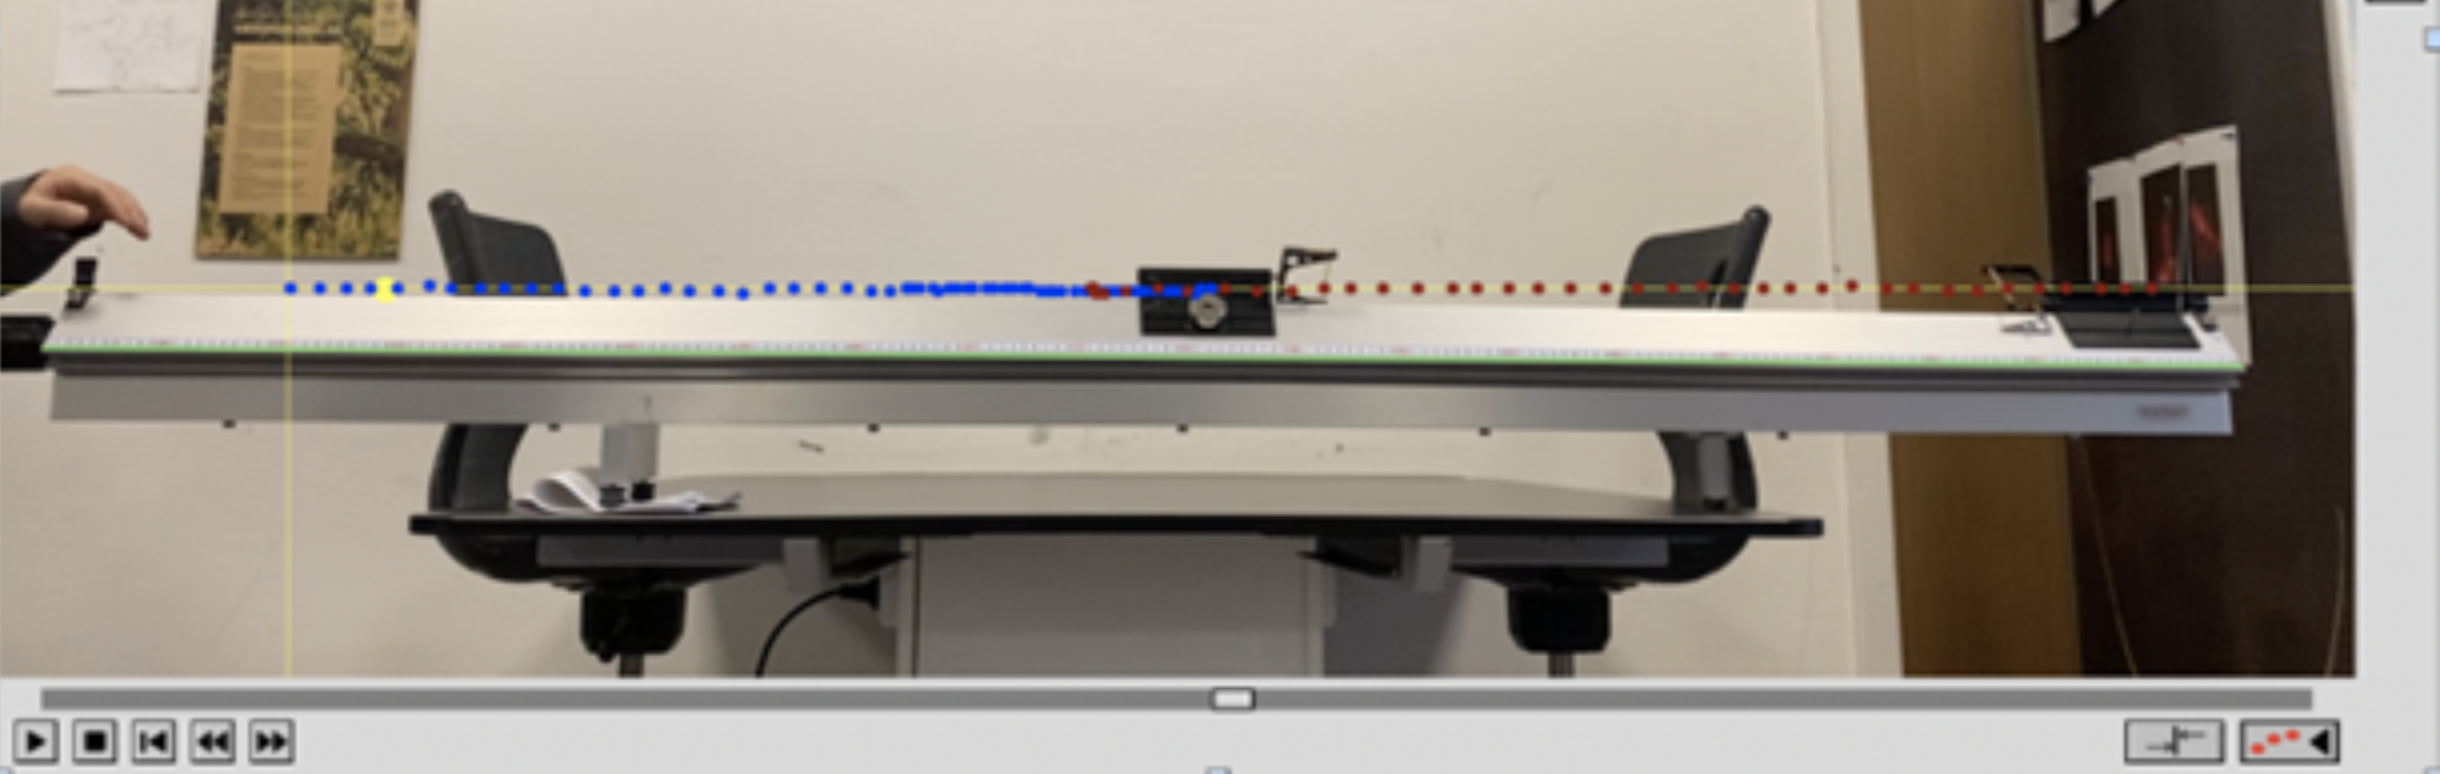
\includegraphics[width=\textwidth]{video-analyse.png}
\end{center}
\caption{Video-analyse lavet i Logger Pro}
\label{fig:video}
\end{figure}
Da vognene kører langsomt nok til, at vi kan se bort fra luftmodstand, og der næsten ingen friktion er, så må de før og efter sammenstødet køre med konstant fart.
Vi kigger da på $(t,x)$-grafen for de to vogne, som ses i \cref{fig:tx}.
Hældningen på grafen før og efter stødet må da være vognenes fart hhv. før og efter stødet, og bestemmes via lineær regression.
\begin{figure}[H]
\begin{center}
  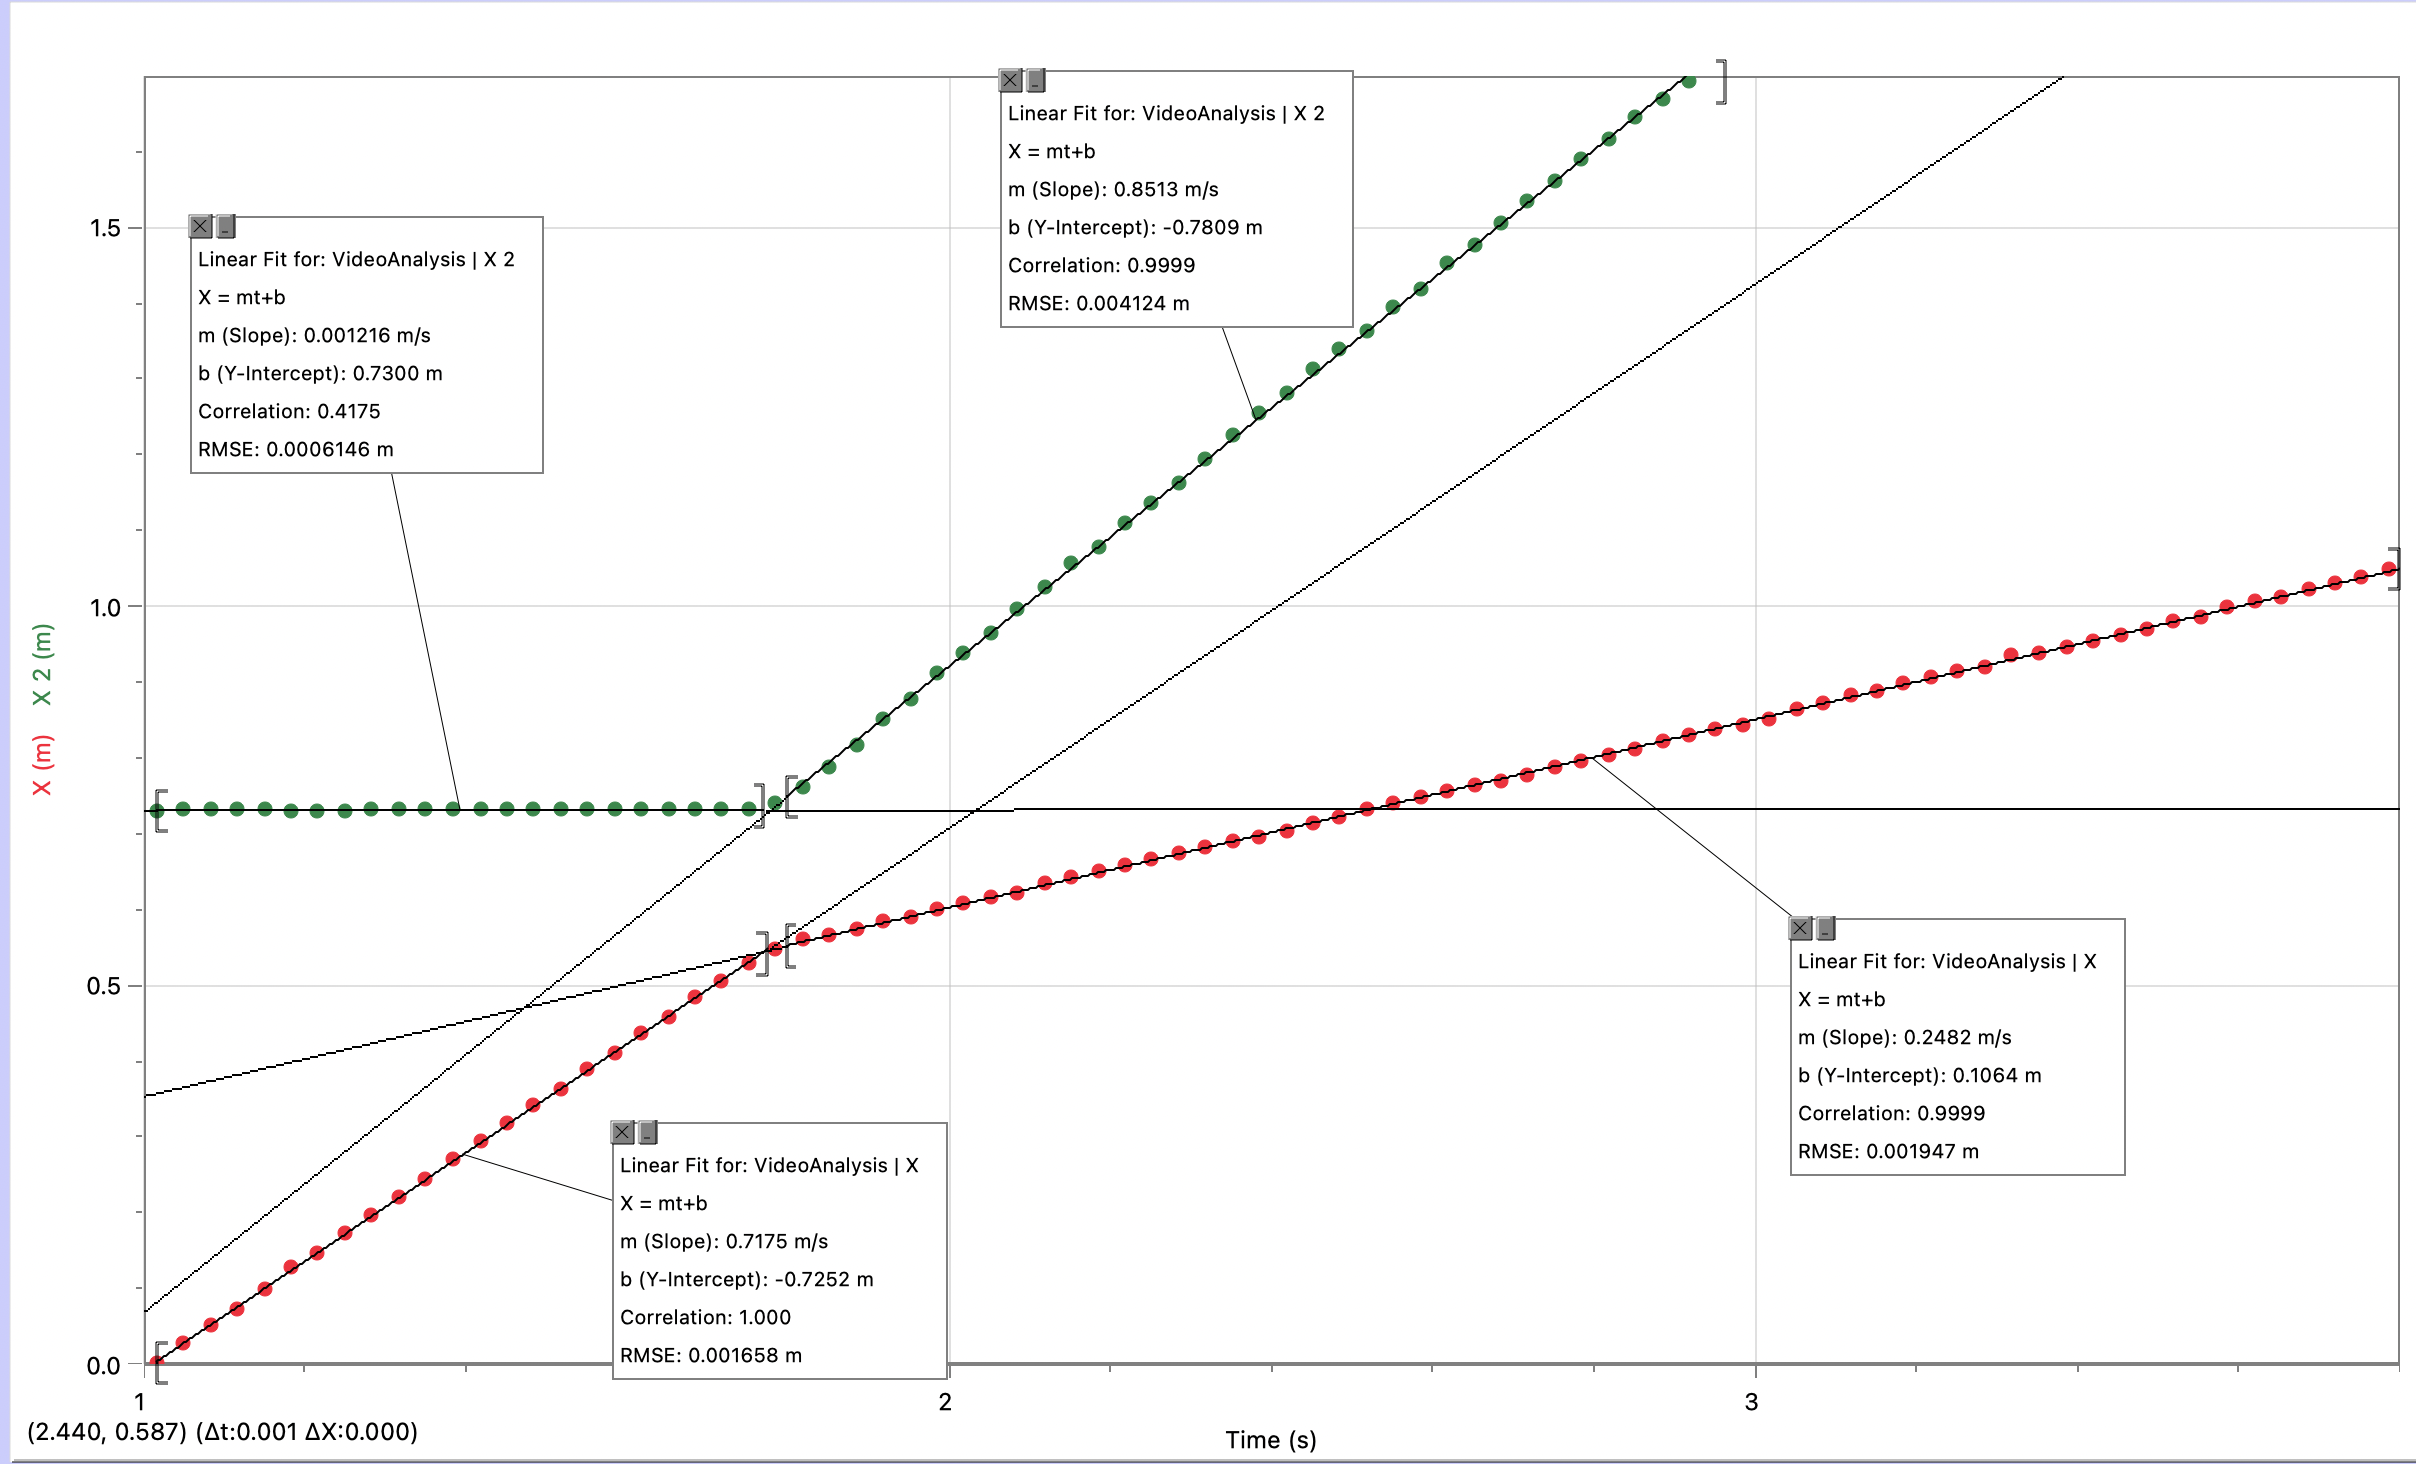
\includegraphics[width=0.8\textwidth]{(t,x).png}
\end{center}
  \caption{Lineær regressioner på $(t,x)$-graferne for de to vogne hhv. før og efter stødet}
\label{fig:tx}
\end{figure}
Tilsvarende gøres i alle andre forsøg for at finde farten på vogn 1, som betegnes $v_1$ før og efter stødet samt farten på vogn 2, som betegnes $v_2$ før og efter stødet. 

Forsøgene inddeles i 3 runder.
Den første runde er "elastisk" stød, hvor vognene kører mod hinanden.
Anden runde er "elastisk" støde, hvor vogn 1 kører ind i vogn 2, der holder stille.
Tredje runder er fuldstændig uelastisk stød, hvor vogn 1 kører ind i vogn 2, der holder stille, og vognene følges ad efter stødet.
Resultaterne og efterbehandlingen for de tre runder ses i \cref{fig:r1}, \cref{fig:r2} og \cref{fig:r3}.
\begin{figure}[H]
\begin{center}
  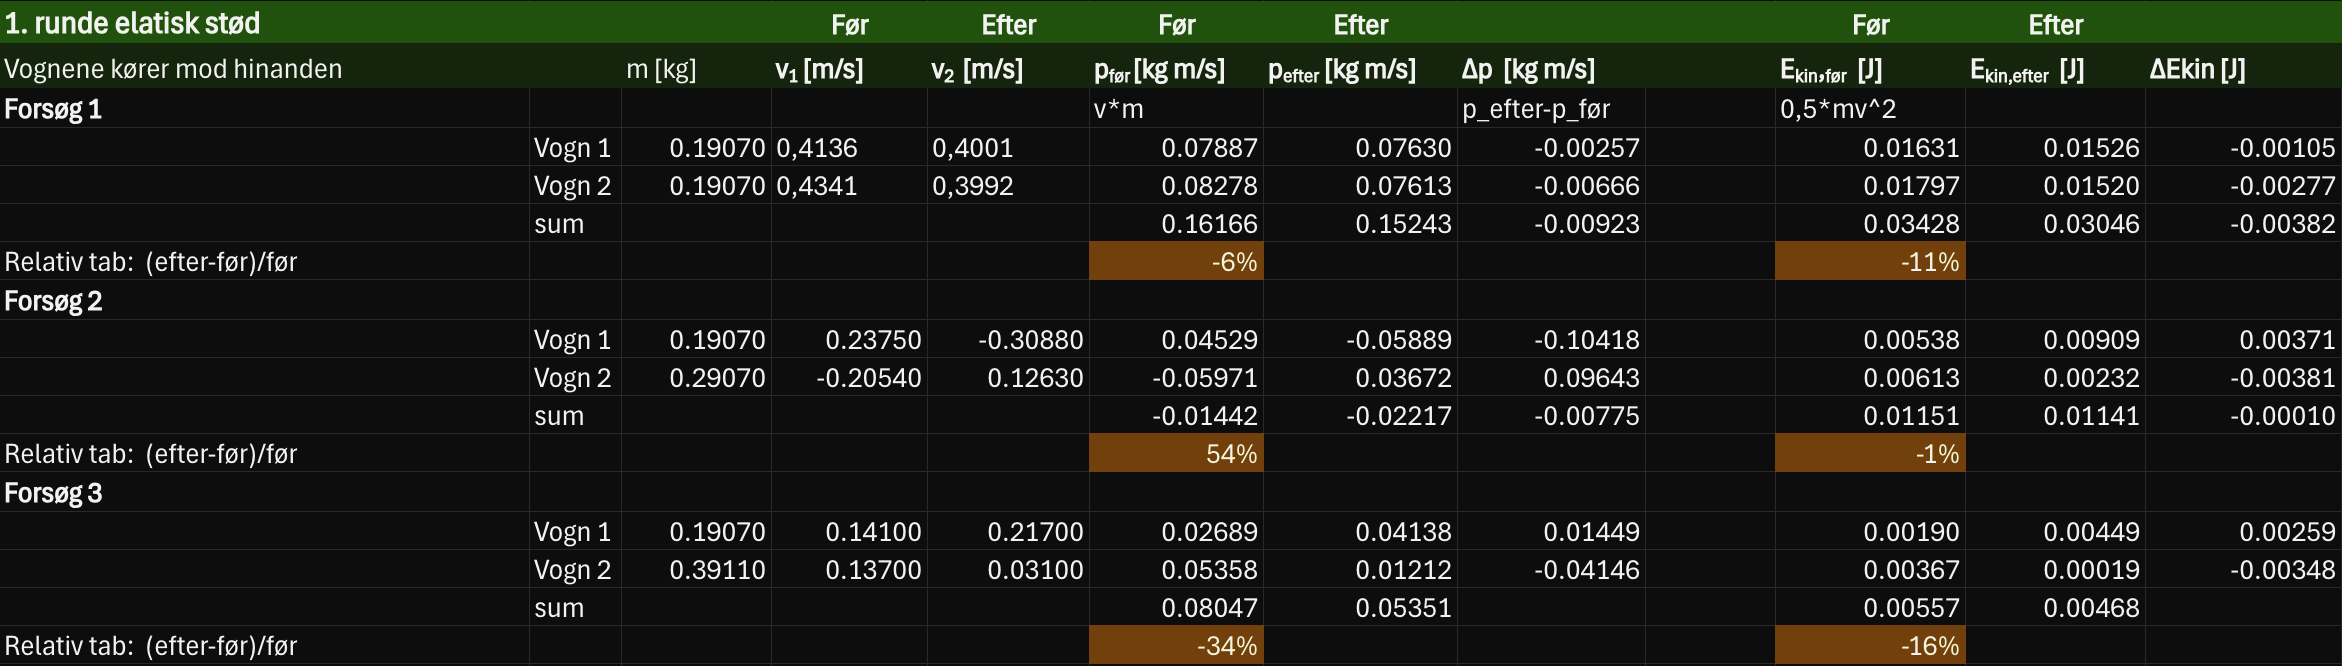
\includegraphics[width=\textwidth]{r1.png}
\end{center}
\caption{Efterbehandling af resultater fra 1. runde i Excel}
\label{fig:r1}
\end{figure}
\begin{figure}[H]
\begin{center}
  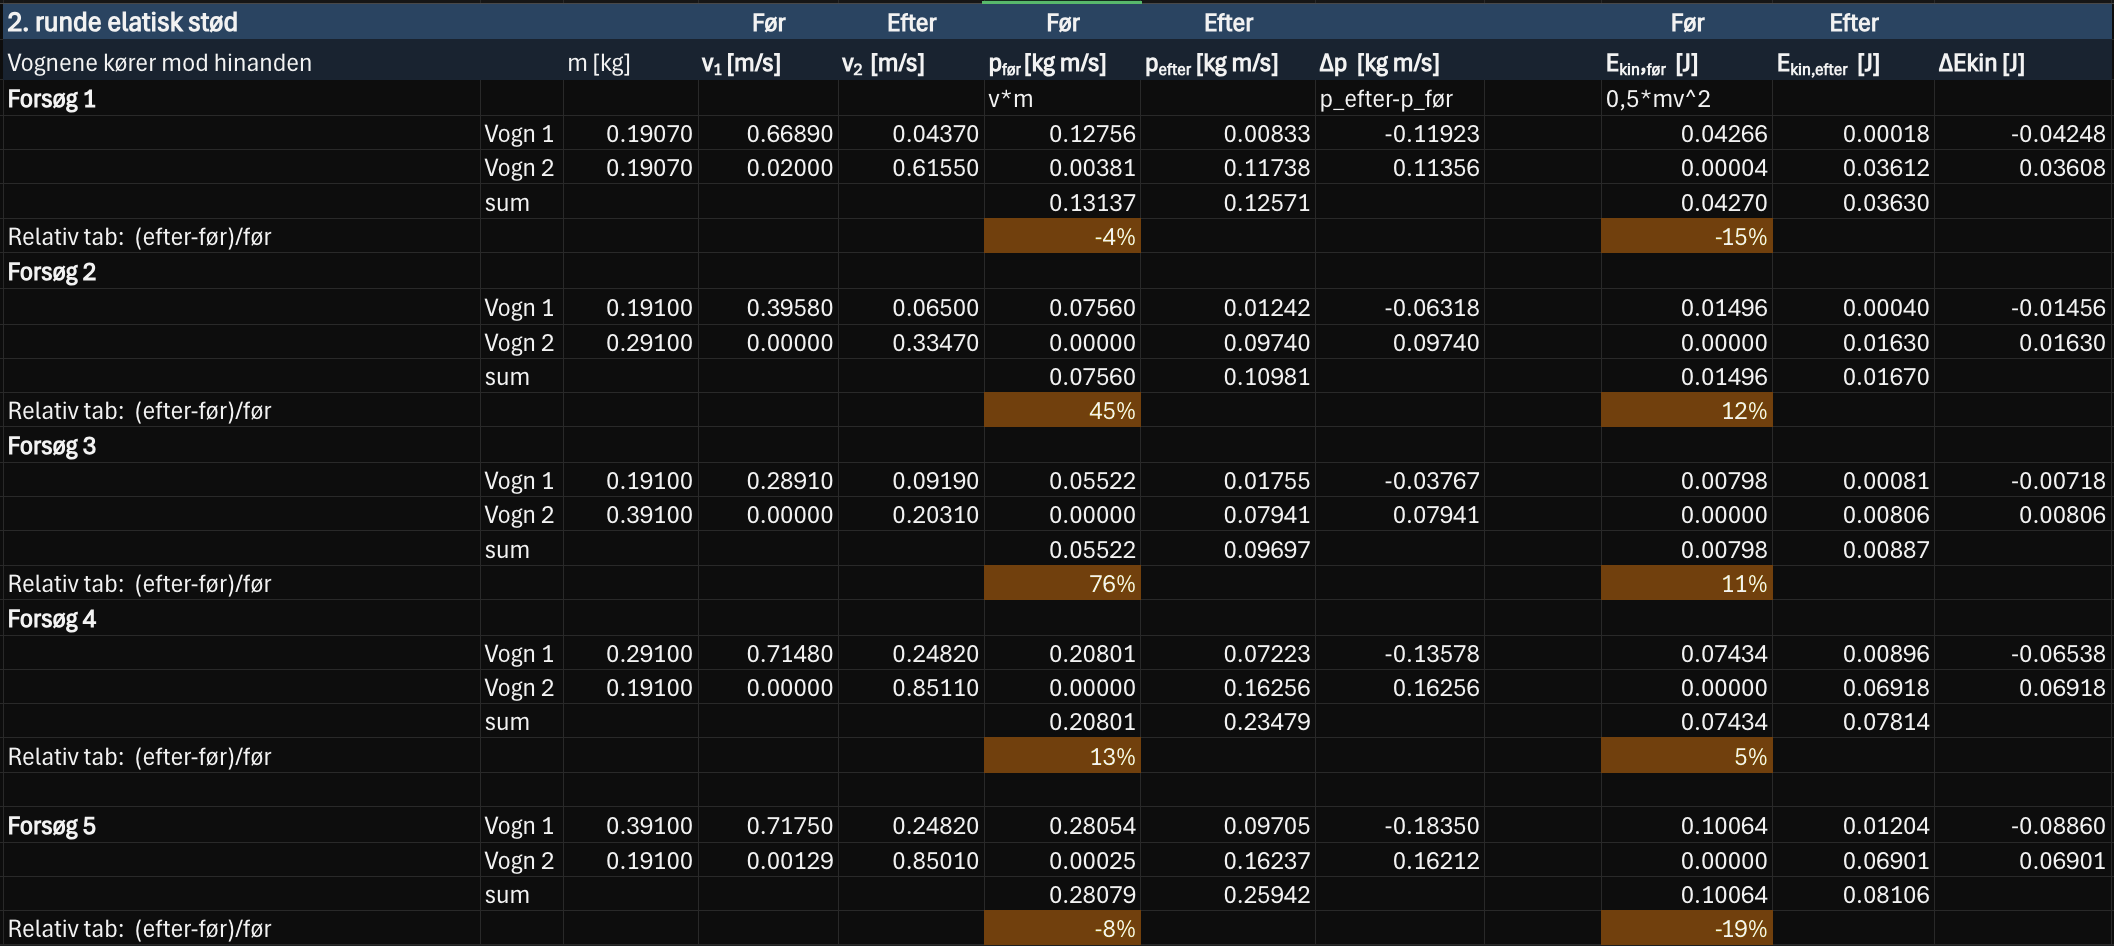
\includegraphics[width=\textwidth]{r2.png}
\end{center}
\caption{Efterbehandling af resultater fra 2. runde i Excel}
\label{fig:r2}
\end{figure}
\begin{figure}[H]
\begin{center}
  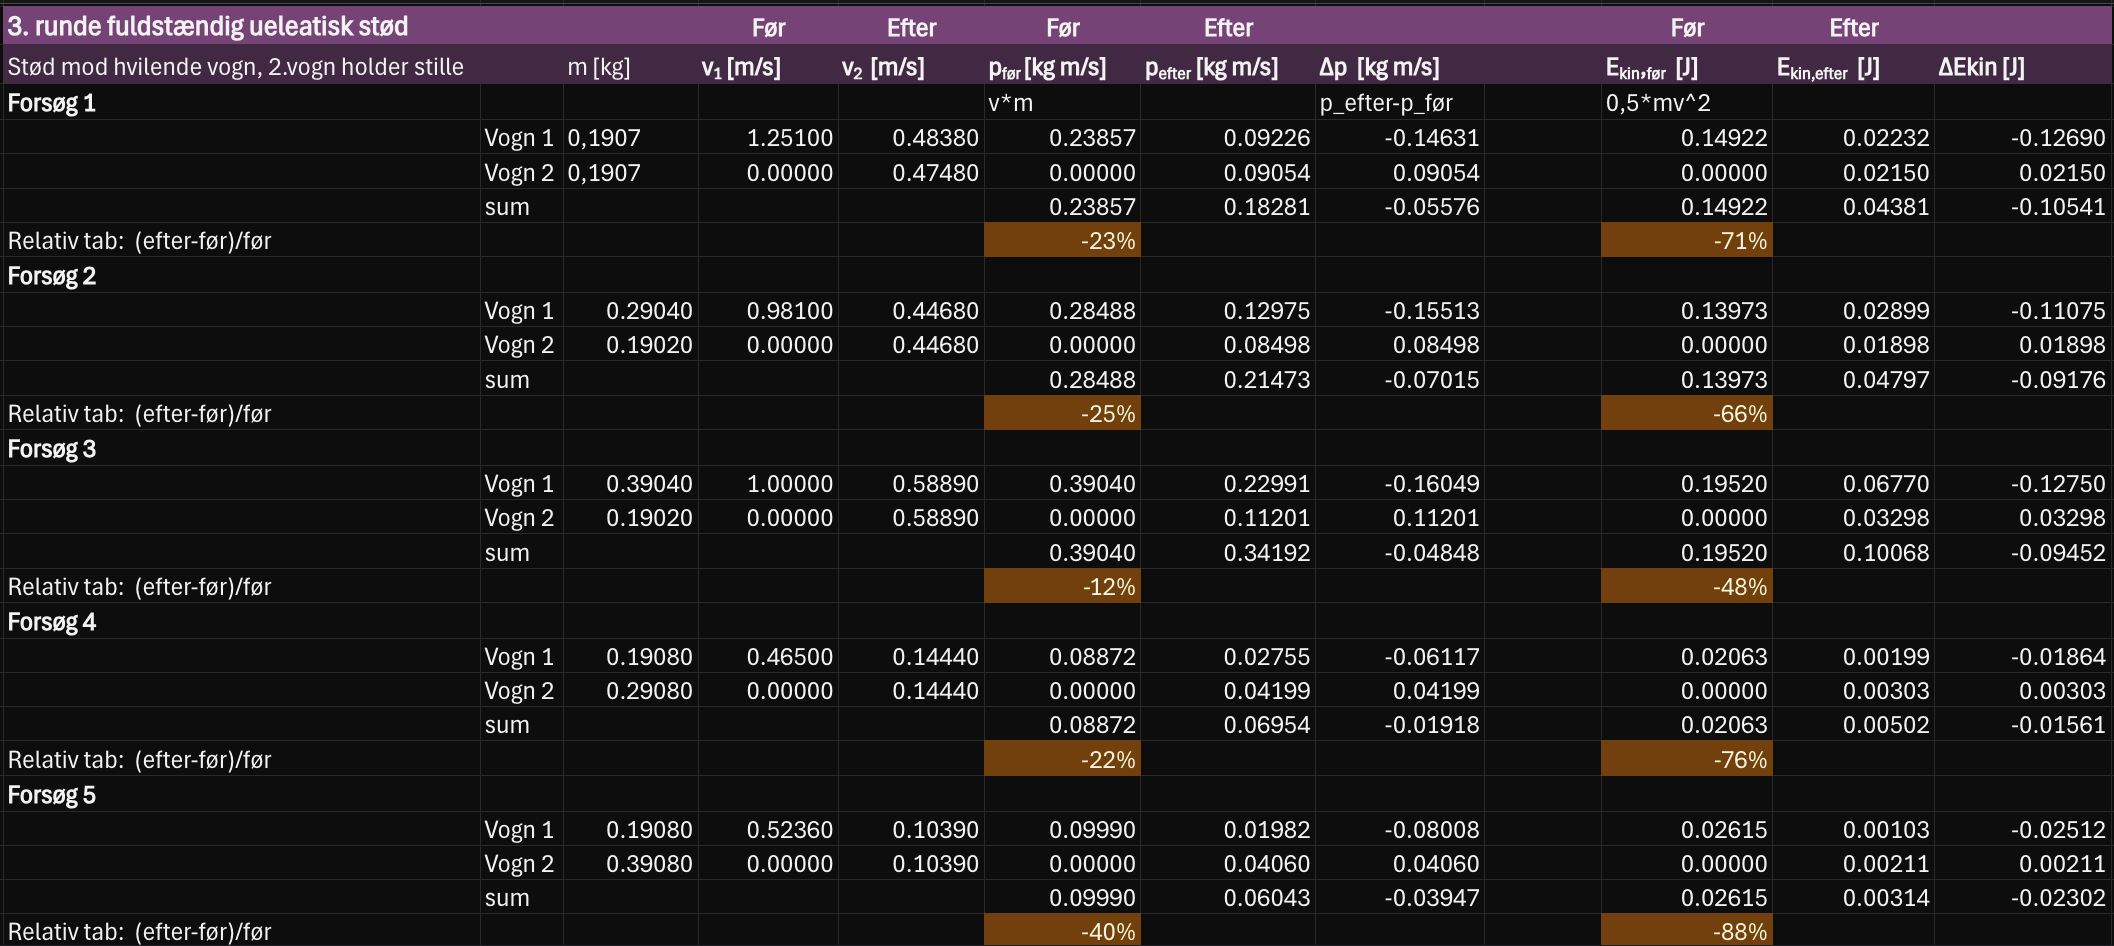
\includegraphics[width=\textwidth]{r3.png}
\end{center}
\caption{Efterbehandling af resultater fra 3. runde i Excel}
\label{fig:r3}
\end{figure}
I tabellerne er det relative tab af bevægelsesmængde og kinetisk energi markeret med orange.
Bemærk, at det "relative tab" regnes som den relative tilvækst, altså vil eksempelvis et tab på den samlede bevægelsesmængde være angivet som negativ.
Vi ser først på, hvorvidt vognenes samlede bevægelsesmængde er bevaret. 
Hvis bevægelsesmængden er fuldstændigt bevaret, så vil det relative tab være på $0 \%$.
Det er dog klart ikke tilfældet ved alle forsøg, da nogle forsøg endda får en relativt stor \textit{tilvækst} i den samlede bevægelsesmængde, selvom den teoretisk burde være bevaret, da vognene kolliderer uden påvirkning af kræfter udefra.
En mulig grund til en \textit{tilvækst} i bevægelsesmængde (altså positivt "relativ tab" her) beskrives under fejlkilder.

Når vi kigger på det gennemsnitlige relative tab af den samlede bevægelsesmængde i \cref{fig:bvm}, ser det dog noget bedre ud.
\begin{figure}[H]
\begin{center}
  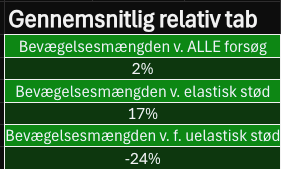
\includegraphics[width=0.5\textwidth]{bvm.png}
\end{center}
\caption{Gennemsnitlige relative tab af bevægelsesmængde regnet med Excel}
\label{fig:bvm}
\end{figure}
Når vi kigger på vognenes samlede kinetiske energi, er den tilnærmelsesvist bevaret ved elastisk stød, hvor den ikke er det ved fuldstændig uelastisk stød.
De gennemstitlige relative tab ses i \cref{fig:kin}.
Per definition er et elastisk stød et stød, hvor de kolliderende partiklers energi efter stødet er lige så stor som før stødet.
Det kan ikke lade sig gøre i virkeligheden, og vores "elastiske" stød kan da formelt set ikke kaldes sådan.
Dog er vores elatiske stød-forsøg meget tæt på at være elastiske.
\begin{figure}[H]
\begin{center}
  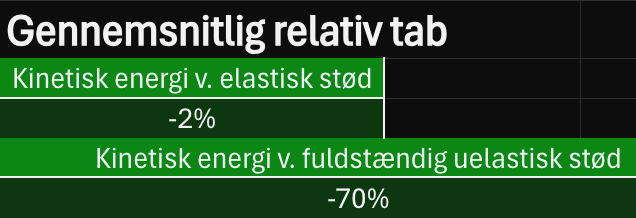
\includegraphics[width=0.7\textwidth]{Ekin.png}
\end{center}
\caption{Gennemsnitlige relative tab af kinetisk energi}
\label{fig:kin}
\end{figure}



\section*{Fejkilder}
Hvis banen ikke er helt i vater, vil den stilleholdende vogn ikke holde helt stille, hvilket vil gøre det "relative tab" større, da farten alligevel angives som 0.
Altså vil tilvæksten i bevægelsesmængde $\Delta p$ være større end den egentlig er. 
Derudover ville eventuelle parallakse-problemer ved filmningen vil have indflydelse på de yderste målinger (tæt på siderne af videoen).

\section*{Konklusion}
Ved støddene er bevægelsesmængden nogenlunde bevaret, og den kinetiske energi er tilnærmelsesvist bevaret ved vores "elastiske" stød, hvor den ikke er bevaret ved de fuldstændig uelastiske stød.


\end{document}
